%%==================================================================%%
%% Author : Tejedo Gonz�lez, Daniel                                 %%
%%          S�nchez Barreiro, Pablo                                 %%
%% Version: 1.0, 22/11/2012                                         %%                   %%                                                                  %%
%% Memoria del Proyecto Fin de Carrera                              %%
%% Planificacion, planificacion                                    %%
%%==================================================================%%

Como en todo proyecto de este tipo, existe un primer paso de documentaci�n y aprendizaje de los diversos conceptos implicados en el mismo. En mi caso, esta tarea conllev� la familiarizaci�n con las L�neas de Producto Software, los �rboles de Caracter�sticas, la Ingenier�a de Lenguajes Dirigida por Modelos y la situaci�n en que se hallaba en ese momento la herramienta Hydra. Una vez culminado este proceso de adquisici�n de informaci�n, que dur� aproximadamente 3 meses, pudimos iniciar la planificaci�n de las tareas a realizar en el proyecto, tal y como se detalla en la figura \ref{figplan}.

\begin{figure}[t]
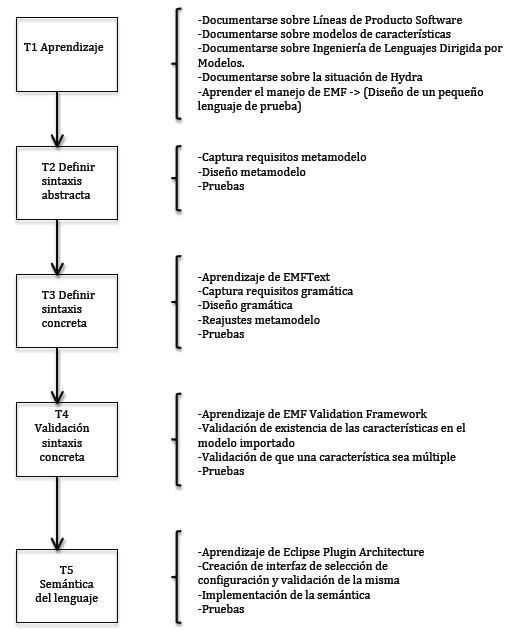
\includegraphics[scale=0.74]{planificacion/planning.jpg}
\caption{Tareas realizadas en este proyecto de fin de carrera}
\label{figplan}
\end{figure}

La tarea 2, definici�n de la sintaxis abstracta, comprende la captura de requisitos del lenguaje que hemos de desarrollar (para as� poder crear el metamodelo de la manera adecuada), dise�o del metamodelo y pruebas de que funciona correctamente. El desarrollo de esta tarea se prolong� durante aproximadamente 3 meses.

La tarea 3, definici�n de la sintaxis concreta, comprende un nuevo aprendizaje, en este caso el de la herramienta para creaci�n de gram�ticas para metamodelos llamada EMFText. Despu�s hubo que hacer una nueva captura de requisitos, menos profunda que la anterior, para poder construir adecuadamente la gram�tica. La construcci�n de la misma tuvo como consecuencia sucesivas pruebas y cambios en el metamodelo hasta dejarlo terminado. Esta tarea tuvo una duraci�n aproximada de 5 meses.

La tarea 4, validaci�n de sintaxis abstracta, comienza con el aprendizaje de una nueva herramienta, el EMF Validation Framework. Tras ello, se construyen los mecanismos necesarios para poder validar que las caracter�sticas a las que queremos aplicar las restricciones existen en el modelo importado, y tambi�n validar que una caracter�stica parseada como m�ltiple (con cardinalidad mayor que 1) sea en efecto m�ltiple en el modelo importado. Esta tarea tuvo una duraci�n aproximada de 2 meses.

La tarea 5, creaci�n de la sem�ntica del lenguaje, comprende la creaci�n de los mecanismos para que las restricciones puedan ser validadas. Es decir, implementar el c�digo que evalua si son ciertas o no, e implementar la interfaz que permite cargar una configuraci�n del modelo. Esta tarea tuvo una duraci�n aproximada de 2 meses.

Todas estas tareas ser�n explicadas m�s en detalle en cap�tulos sucesivos.

La metodolog�a de desarrollo de este proyecto vino impuesta por la t�cnica de Ingenier�a de Lenguajes Dirigida por Modelos. Es decir, no se pudo aplicar ninguna de las t�cnicas cl�sicas como "metodolog�a incremental", pues las peculiares caracter�sticas de la ingenier�a de modelos impiden que eso sea viable. 